\documentclass[12pt]{article}
\usepackage{amsmath}
\usepackage{amssymb}
\usepackage{graphicx}
\usepackage[margin=1in]{geometry}
\newcommand{\del}{\nabla}
\begin{document}

\title{Kronecker Graphs for Modelling Linguistic Data}
\author{Howon Lee (howonlee)}
\maketitle

\section{Introduction}

An important statistical regularity in language is Zipf's law, which says that given some corpus of natural language, the frequency of any word is inversely proportional to its rank on the frequency table. However remarkable it may be, however, it is not a statement about the structure of language. This is because it holds for corpuses as bags of words which have frequencies, not as linguistic entities which have internal structure. \cite{smallworldlang}

One important language model which is used in many places which incorporates some aspect of linguistic structure, notably without specifying it, is the n-gram, which creates a Markov model of language, taking the semi-Markov assumption that the only context needed to reproduce a word is the past $n$ words. This is of interest, because it turns out that thinking of a corpus as a graph of words and the order-one and order-two relations between words, as bigram and trigram models do, reveals many small-world properties in the structuring of words in corpuses.

In this paper we deal, therefore, with the problem of using and adapting already existing algorithms for creating small world nets by creating a parsimonious model of language with Kronecker graphs that respects these network properties of words as they currently exist.

\section{Literature Review}

We review MEJ Newman's \emph{Power laws, Pareto Distributions and Zipf's law}\cite{mejpowerlaw}, J. Leskovec and C. Faloutsos's \emph{Scalable Modeling of Real Graphs using Kronecker Multiplication}\cite{kronfit}, and RF Cancho and RV Sole's \emph{The Small World of Human Language}\cite{smallworldlang}.

\subsection{MEJ Newman}
MEJ Newman's paper is a review and introduction to power laws, which are notable for being found in very many domains across nature, and for the unhelpfulness of their first and second moments. That is, the number of inhabitants of the mean city is on the order of $10^3$, but that doesn't tell you about the existence of Tokyo. There are many pitfalls in the estimation of power laws, especially in the least mean square estimation, which gets systematic errors even on synthetic data, and many possible origins of power law phenomena, which are listed: two important ones are Yule processes and critical phenomena.

A particular point of interest is the introduction to a possible information-theoretic origin of Zipf's law. MEJ Newman reviews a possible origin of power law phenomena in language due to Miller\cite{gamiller}. Miller's argument goes like this: imagine a monkey typing on a typewriter, delimiting words with some probability and writing a random letter with some uniform probability. Then, this approximates an exponential distribution of frequency of a word $x$ with number of letters $y$. But the number of possible words goes up exponentially with $y$ also, making the distribution of frequencies a combination of exponentials, which ends up being a power law. This is a simplistic argument, but can be made less simplistic in talking about arbitrary information in bits instead of symbols in the normal alphabet.
. 
\subsection{MEJ Newman Discussion}

As a review paper, there is not any original work in the paper: it must be criticized in whether the distribution of subjects in the review cleave closely to the importance the field should give to the respective subjects. To that end, a strong point of the paper is its covering most things which were known about the power law phenomena at the time, and being skeptical about the general trend of plotting some distribution, finding a fat tail, and declaring that the phenomenon respected a power law: that skepticism is continued in C. Shalzi's paper\cite{cosma}, and will be used in our fractal analysis, especially in avoiding least square fits and plotting with CDF's.

The main point of contention we have with the paper is in presenting GA Miller's monkey on a typewriter argument as the purported source of Zipf's law. This is because this theory is only compatible with a random typewriter with no structure. That is, to condition on the previous letters or words gives no information for the generation of the typewriter model, except that the example of Shannon's communication game, that of guessing the next word based upon the previous words in a communication, implies this sort of conditional structure. And humans in real life can play this communication game. This is probably more of a contention with Miller's paper than with MEJ Newman's.

\subsection{J Leskovec, C. Faloutsos}
A possible model of small world graphs is the stochastic Kronecker graph, which is a sample from a distribution over graphs. The distribution is created by drawing a fractal over an adjacency matrix using the Kronecker product operation. The important thing about this model is that it tries to simultaneously fulfill the many observed properties of small world graphs, not just the heavy tail for indegree and outdegree, but also the heavy tail for scree plots, the densification power law, and small diameters, all at the same time.

The novel contribution of this paper is to note that the parameters for that distribution can be fitted with an algorithm described in the paper. KronFit is a gradient descent algorithm, but is much, much faster than other such algorithms for graphs like the exponential random graph. This is because it uses MCMC to assign node labels, avoiding that combinatorial explosion, and because it uses the sparsity of the small world graph to start with the likelihood of an empty graph and adjust for the edges that exist, in time linear to the number of edges instead of quadratic to the number of nodes. The number of parameters is determined using a BIC metric. Every part of this algorithm can and should be done when the whole matrix does not fit in memory.

There are also real interpretations of the Kronecker product process in the structure and creation of graphs. One intuition is that networks are hierarchically organized into communities, which grow recursively, creating miniature copies of themselves. Another interpretation is to say that each node is described by a sequence of categorical features, and the probability of two nodes linking depends on the product of individual attribute similarities, which allows modelling of homophily and heterophily at the same time.

\subsection{J Leskovec, C. Faloutsos discussion}

One important point to re-iterate is that one suggested usage for the Kronecker fitting algorithm is for compression of graphs. This is important, because whenever we hear "compression" we should smell "machine learning", because any system of compression can be used for prediction, by finding the symbol that compresses best given the history of the data \cite{mlcompression}.

There is another work which notes that local search (viz., decentralized search) cannot efficiently find paths through Kronecker graphs. This is a large lacuna in the claim that Kronecker graphs are an attempt to model every aspect of how small world networks work at once\cite{stochkrongraph}.

One omission must be noted. Both interpretations of the Kronecker product process in the structure and creation of the Kronecker graphs are recursive in nature, in this case fractally self-similar. Therefore, the Kronecker graph model implicitly tells a fractal story about the creation of any small-world net which one models with it, that its construction is fractal and therefore that the existing machinery of fractal analysis can be used upon it.

\subsection{RF Cancho, RV Sole}
Cancho and Sole's paper talk about the implicit statistical regularities in a small world net made from the co-occurrence network of words in sentences. Instead of talking about syntactic structure in sentences, they investigate the statistical structure of these mere co-occurrences, with the admittedly simplistic assumption that the trigrams and bigrams are correlated.

Why? Four reasons. It's much easier to get those link structures automatically, as opposed to syntactic ones. They don't know what types of links there are in the structures of words, but just having the propinquity of words will capture almost every type. They are not interested in all the links, so looking at whole sentences will not be as productive. Long-distance syntactic links imply the existence of lower-distance syntactic links, but not vice versa.

Looking at the graph created in this way, they find small-world properties like high clustering coefficient, small diameter and power law degree distribution. They hypothesize that this leads to words that exist to speed up navigation in this small world, words like "and", "the", "of", "in", which do not contribute meaning but structure to grammar. They also hypothesize that the disfluency caused in agrammatism is caused by disruption to this small world.

\subsection{RF Cancho, RV Sole discussion}

Because the RF Cancho and RV Sole paper was from 2001, there exist some properties of small world graphs which were first published afterwards and therefore for good reason were not examined. For example, the densification power law\cite{densificationpowerlaw} and skewed network values\cite{netvalskew} are properties reviewed in the Kronecker graph article but not in this paper, among others. So figures 1 and 2 are an analysis of those two properties using a 1st-order word net (bigram). In this case, this is a directed and not an undirected graph. KS test for the densification versus $x^{1.14}$ has p>0.1. %%% skew and densification power law cites

\begin{figure}
  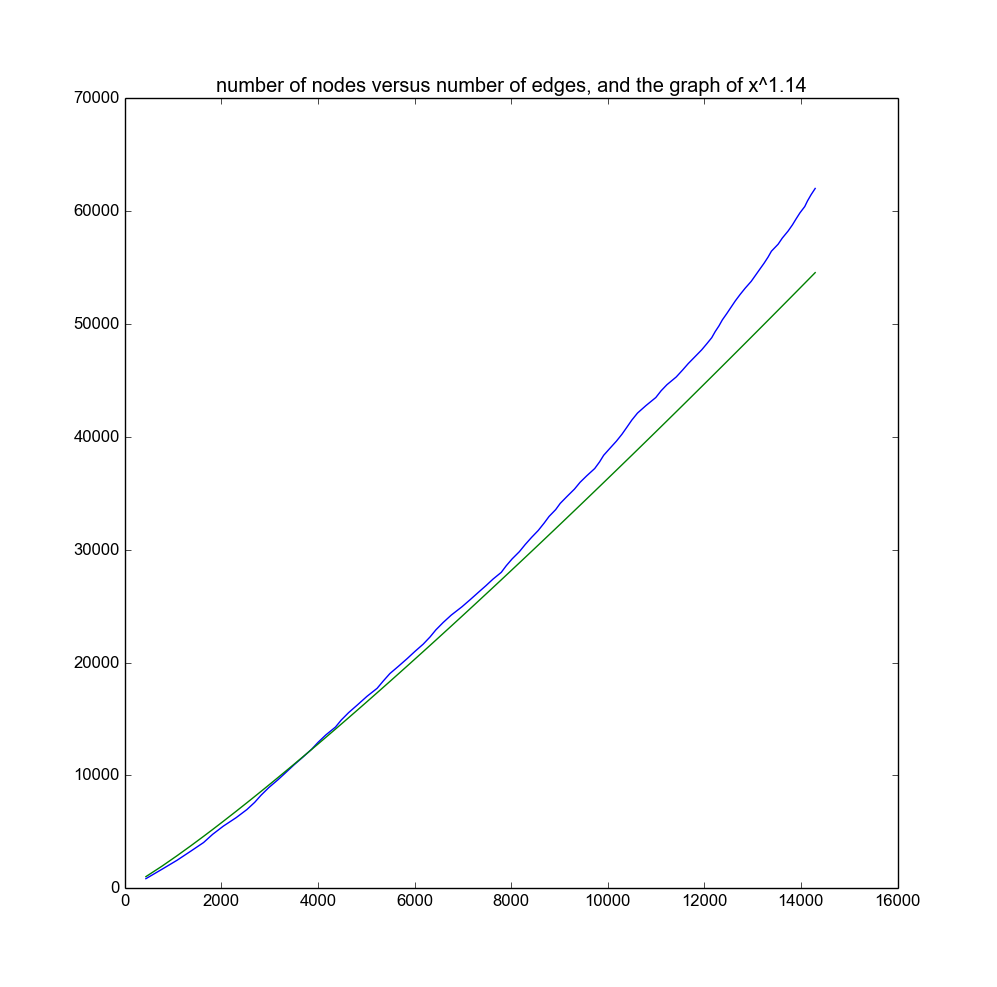
\includegraphics[width=0.5\textwidth]{densification_plot.png}
\end{figure}

\begin{figure}
  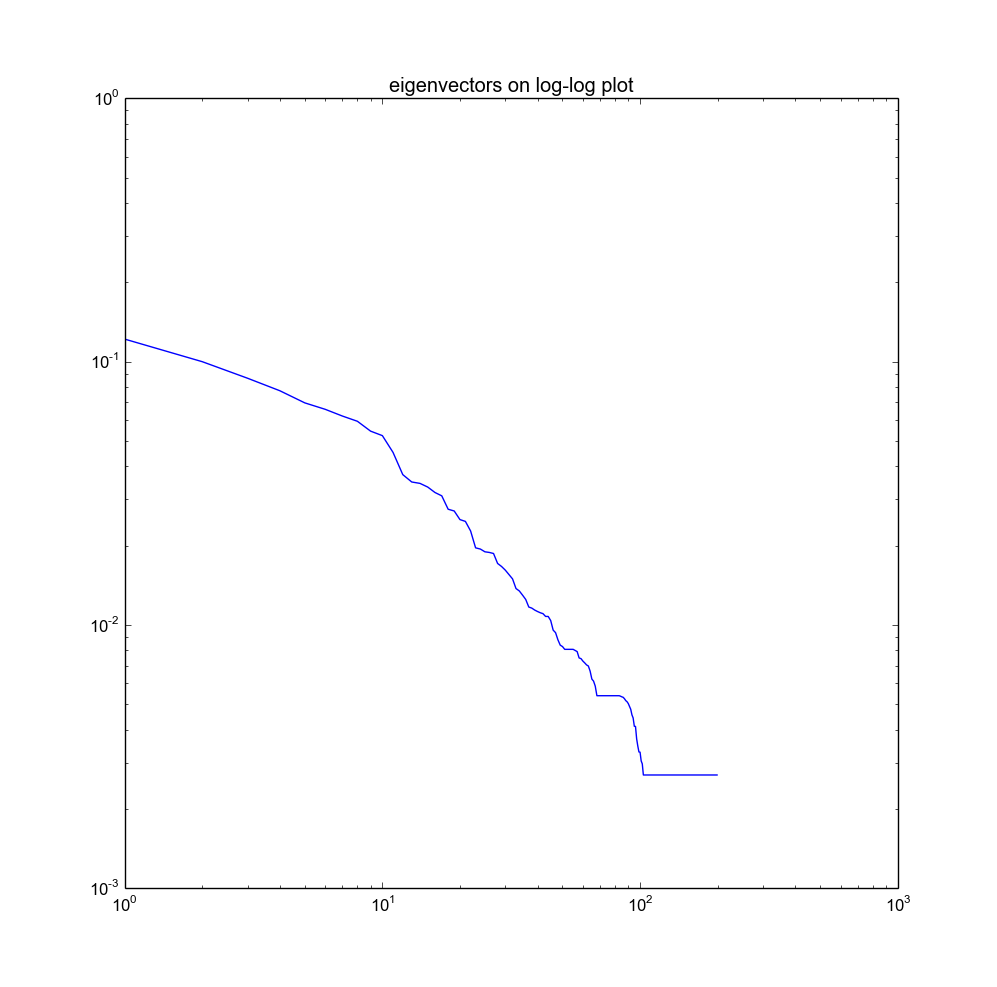
\includegraphics[width=0.5\textwidth]{eigenvector_loglog.png}
\end{figure}

There is ample room for criticizing the decision to say that two words are linked to each other if they are within two words of each other in a corpus. However, I suspect that there is a fairly strong argument for looking at a limited number of juxtaposed words when building such a net, analogous to the argument for only looking at a limited number of scales of resolution when investigating a power law phenomena. That is, fractals are mathematical structures but the real life objects which obey fractal properties only obey them at certain levels, with a lower and upper cutoff in size \cite{fractalcutoffs}

They are missing a practical application for the language model which is implicit in their description of the properties of the small world, because unlike in some other fields creating a model for language is useful in real tasks. We know that humans solve the inverse problem for languages in some way, because there has to be teaching for the learning of a specific language. However, this is not true in many other power-law distributed domains: \emph{Only fools, charlatans and liars predict earthquakes} \cite{richter}. Therefore, there should be room for leveraging this finding that corpus lexicons are characterized by small-world networks language model.

\subsection{Brainstorm}

We should bring forward the idea of a structure of the words in a natural corpus, and we should bring forward the idea that it is a small-world net. Therefore, we should consider modelling using the parameters of the stochastic Kronecker graph as a very parsimonious explanation of such n-gram data. We should also play with the assumptions of the model, since the stochastic Kronecker graph assumes that the weights of the distribution over graphs is fractally distributed over the adjacency matrix.

\section{Project Proposal}

\subsection{Introduction and Problem}
If we take the central thesis of RF Cancho and RF Sole's work to be true, then word networks are small world networks. Therefore, they should be able to be fitted to parameters for a Kronecker distribution, which would compress the language graph to a very few parameters. It should be investigated whether these parameters, this model has any value as a language model. It should also be investigated whether the secondary implicit assumption that the Kronecker model has, that the adjacency matrix of this particular small-world net has fractal structure, is borne out in the data.

Having a language model gives us a tool which is used in many places in NLP, and therefore we should use this model, construed as a language model, in some of the existing NLP tasks that use language model. And if the fractal structure assumption is borne out, that also gives us a feature of corpus data, which we should investigate the use of in a simple authorship attribution task (the task of categorizing a text of unknown provenance to an author) or other simple corpus identification task.
\subsection{Data}
Medium-sized and large corpuses of words are fairly easy to get. We will use the Brown NLTK corpus for development, and then take advantage of the many corpuses in NLTK to attempt the authorship measure, in particular the Gutenberg corpus.
\subsection{Evaluation}
Perplexity is an easy development measure of the generator's goodness. Of course, it's a bad approximation of anything we care about in the generalization performance. We should therefore also do a simple and a more complex task with the language model, such as next-word generation and spell-checking, and evaluate the goodness by a held-out test set and also by examination of the results.

There may also be an interesting investigation possible of fractal dimension \cite{fractaldim} and lacunarity \cite{lacunarity} in the data itself. That is, implicit in the Kronecker graph model is an assumption that the network's adjacency matrix can be treated as a fractal: we should run as far as we can with this assumption, and see if fractal measures of this kind are meaningful and useful as features of the corpus. To this end, we will test an authorship attribution task with standard machine learning algorithms: the specific machine learning algorithm in this case should be less important than ascertaining the fact of whether fractal dimension and lacunarity are important features.

\begin{thebibliography}{99}
%%%
%%% PUT IN CITATIONS
%%%
  \bibitem{smallworldlang}
  \bibitem{kronfit}
  \bibitem{mejpowerlaw}
  \bibitem{fractaldim}
  \bibitem{lacunarity}
  \bibitem{nltk}
  \bibitem{richter}
  \bibitem{fractalcutoffs}
  \bibitem{netvalskew}
  \bibitem{densificationpowerlaw}
  \bibitem{stochkrongraph}
  \bibitem{mlcompression}
  \bibitem{cosma}
  \bibitem{gamiller}
\end{thebibliography}


\end{document}
